\documentclass[11pt,a4paper]{article}

\usepackage{Act}


\begin{document}
\newcommand{\ModeExercice}{
% Traduction des noms pour le package exercise
\renewcommand{\ExerciseName}{Exercice}
\renewcommand{\thesubQuestion}{\theQuestion.\alph{subQuestion}}
\renewcommand{\AnswerName}{Réponses à l'exercise }
}
\newcommand{\Fiche}[2]{\lhead{\textbf{{\sc #1}}}
\rhead{Niveau: \textbf{#2}}
\cfoot{}}
\definecolor{cfond}{gray}{0.4}
\renewcommand{\thealgocf}{}

\newcommand{\ModeActivite}{
% Traduction des noms pour le package exercise
\renewcommand{\ExerciseName}{Activité}
}
% Réglages de la mise en forme des exercices 
\renewcommand{\ExerciseHeaderTitle}{\ExerciseTitle}
\renewcommand{\ExerciseHeaderOrigin}{\ExerciseOrigin}
% Un : sépare le numéro de l'exerice de son titre ... si le titre existe. On utilise Origine pour placer les pictogrammes en fin de ligne
\renewcommand{\ExerciseHeader}{\ding{113} \textbf{\sffamily{\ExerciseName \ \ExerciseHeaderNB}} \ifthenelse{\equal{\ExerciseTitle}{\empty}}{}{:} \textit{\ExerciseHeaderTitle} \hfill \ExerciseHeaderOrigin}
\renewcommand{\ExePartHeader}{\quad {\footnotesize \ding{110}} \textbf{Partie \textbf{\ExePartHeaderNB}} : \ExePartName}


% Mode Concours
\newcommand{\ModeConcours}{
   \newcounter{qconcours}
   \setcounter{qconcours}{1}
   \renewcommand{\ExerciseName}{Exercice}
   \renewcommand{\ExerciseHeaderTitle}{\ExerciseTitle}
\renewcommand{\ExerciseHeaderOrigin}{\ExerciseOrigin}
\renewcommand{\ExerciseHeader}{\ding{113} \textbf{\sffamily{\ExerciseName \ \ExerciseHeaderNB}} \ifthenelse{\equal{\ExerciseTitle}{\empty}}{}{:} \textit{\ExerciseHeaderTitle} \hfill \ExerciseHeaderOrigin}
\renewcommand{\QuestionNB}{\textbf{Q\arabic{qconcours}--}\ \addtocounter{qconcours}{1}}}

\newcommand{\noeud}[1]{\Tr{\fbox{\tt #1}}}
\newcommand{\FPATH}{/home/fenarius/Travail/Cours/cpge-info/docs/mp2i/}
\newcommand{\spath}[2]{\FPATH Evaluations/#1/#1#2}
\definecolor{codebg}{gray}{0.90}
\newcommand{\inputpartOCaml}[5]{\begin{mdframed}[backgroundcolor=codebg] \inputminted[breaklines=true,fontsize=#3,linenos=true,highlightcolor=fluo,tabsize=2,highlightlines={#2},firstline=#4,lastline=#5,firstnumber=1]{OCaml}{#1} \end{mdframed}}
\newcommand{\inputpartPython}[5]{\begin{mdframed}[backgroundcolor=codebg] \inputminted[breaklines=true,fontsize=#3,linenos=true,highlightcolor=fluo,tabsize=2,highlightlines={#2},firstline=#4,lastline=#5,firstnumber=1]{python}{#1} \end{mdframed}}
\newcommand{\inputpartC}[5]{\begin{mdframed}[backgroundcolor=codebg] \inputminted[breaklines=true,fontsize=#3,linenos=true,highlightcolor=fluo,tabsize=2,highlightlines={#2},firstline=#4,lastline=#5,firstnumber=1]{c}{#1} \end{mdframed}}
\newcommand{\inputC}[2]{\begin{mdframed}[backgroundcolor=codebg] \inputminted[breaklines=true,fontsize=#2,linenos=true,highlightcolor=fluo,tabsize=2]{c}{#1} \end{mdframed}}
\newminted[langageC]{c}{linenos=true,escapeinside=``,highlightcolor=fluo,tabsize=2}
\newminted[python]{python}{linenos=true,escapeinside=``,highlightcolor=fluo,tabsize=4}
\BeforeBeginEnvironment{minted}{\begin{mdframed}[backgroundcolor=codebg,skipabove=0cm]}
   \AfterEndEnvironment{minted}{\end{mdframed}}

% Font light medium et bold pour tt :
\newcommand{\ttl}[1]{\ttfamily \fontseries{l}\selectfont #1}
\newcommand{\ttm}[1]{\ttfamily \fontseries{m}\selectfont #1}
\newcommand{\ttb}[1]{\ttfamily \fontseries{b}\selectfont #1}

%QCM de NSI \QNSI{Question}{R1}{R2}{R3}{R4}
\newcommand{\QNSI}[5]{
#1
\begin{enumerate}[label=\alph{enumi})]
\item #2
\item #3
\item #4
\item #5
\end{enumerate}
}



\definecolor{grispale}{gray}{0.95}
\newcommand{\htmlmode}{\lstset{language=html,numbers=left, tabsize=2, frame=single, breaklines=true, keywordstyle=\ttfamily, basicstyle=\small,
   numberstyle=\tiny\ttfamily, framexleftmargin=0mm, backgroundcolor=\color{grispale}, xleftmargin=12mm,showstringspaces=false}}
\newcommand{\pythonmode}{\lstset{language=python,numbers=left, tabsize=4, frame=single, breaklines=true, keywordstyle=\ttfamily, basicstyle=\small,
   numberstyle=\tiny\ttfamily, framexleftmargin=0mm, backgroundcolor=\color{grispale}, xleftmargin=12mm, showstringspaces=false}}
\newcommand{\bashmode}{\lstset{language=bash,numbers=left, tabsize=2, frame=single, breaklines=true, basicstyle=\ttfamily,
   numberstyle=\tiny\ttfamily, framexleftmargin=0mm, backgroundcolor=\color{grispale}, xleftmargin=12mm, showstringspaces=false}}
\newcommand{\exomode}{\lstset{language=python,numbers=left, tabsize=2, frame=single, breaklines=true, basicstyle=\ttfamily,
   numberstyle=\tiny\ttfamily, framexleftmargin=13mm, xleftmargin=12mm, basicstyle=\small, showstringspaces=false}}
   
   
  \lstset{%
        inputencoding=utf8,
        extendedchars=true,
        literate=%
        {é}{{\'{e}}}1
        {è}{{\`{e}}}1
        {ê}{{\^{e}}}1
        {ë}{{\¨{e}}}1
        {É}{{\'{E}}}1
        {Ê}{{\^{E}}}1
        {û}{{\^{u}}}1
        {ù}{{\`{u}}}1
        {ú}{{\'{u}}}1
        {â}{{\^{a}}}1
        {à}{{\`{a}}}1
        {á}{{\'{a}}}1
        {ã}{{\~{a}}}1
        {Á}{{\'{A}}}1
        {Â}{{\^{A}}}1
        {Ã}{{\~{A}}}1
        {ç}{{\c{c}}}1
        {Ç}{{\c{C}}}1
        {õ}{{\~{o}}}1
        {ó}{{\'{o}}}1
        {ô}{{\^{o}}}1
        {Õ}{{\~{O}}}1
        {Ó}{{\'{O}}}1
        {Ô}{{\^{O}}}1
        {î}{{\^{i}}}1
        {Î}{{\^{I}}}1
        {í}{{\'{i}}}1
        {Í}{{\~{Í}}}1
}

%tei pour placer les images
%tei{nom de l’image}{échelle de l’image}{sens}{texte a positionner}
%sens ="1" (droite) ou "2" (gauche)
\newlength{\ltxt}
\newcommand{\tei}[4]{
\setlength{\ltxt}{\linewidth}
\setbox0=\hbox{\includegraphics[scale=#2]{#1}}
\addtolength{\ltxt}{-\wd0}
\addtolength{\ltxt}{-10pt}
\ifthenelse{\equal{#3}{1}}{
\begin{minipage}{\wd0}
\includegraphics[scale=#2]{#1}
\end{minipage}
\hfill
\begin{minipage}{\ltxt}
#4
\end{minipage}
}{
\begin{minipage}{\ltxt}
#4
\end{minipage}
\hfill
\begin{minipage}{\wd0}
\includegraphics[scale=#2]{#1}
\end{minipage}
}
}

%Juxtaposition d'une image pspciture et de texte 
%#1: = code pstricks de l'image
%#2: largeur de l'image
%#3: hauteur de l'image
%#4: Texte à écrire
\newcommand{\ptp}[4]{
\setlength{\ltxt}{\linewidth}
\addtolength{\ltxt}{-#2 cm}
\addtolength{\ltxt}{-0.1 cm}
\begin{minipage}[b][#3 cm][t]{\ltxt}
#4
\end{minipage}\hfill
\begin{minipage}[b][#3 cm][c]{#2 cm}
#1
\end{minipage}\par
}



%Macros pour les graphiques
\psset{linewidth=0.5\pslinewidth,PointSymbol=x}
\setlength{\fboxrule}{0.5pt}
\newcounter{tempangle}

%Marque la longueur du segment d'extrémité  #1 et  #2 avec la valeur #3, #4 est la distance par rapport au segment (en %age de la valeur de celui ci) et #5 l'orientation du marquage : +90 ou -90
\newcommand{\afflong}[5]{
\pstRotation[RotAngle=#4,PointSymbol=none,PointName=none]{#1}{#2}[X] 
\pstHomO[PointSymbol=none,PointName=none,HomCoef=#5]{#1}{X}[Y]
\pstTranslation[PointSymbol=none,PointName=none]{#1}{#2}{Y}[Z]
 \ncline{|<->|,linewidth=0.25\pslinewidth}{Y}{Z} \ncput*[nrot=:U]{\footnotesize{#3}}
}
\newcommand{\afflongb}[3]{
\ncline{|<->|,linewidth=0}{#1}{#2} \naput*[nrot=:U]{\footnotesize{#3}}
}

%Construis le point #4 situé à #2 cm du point #1 avant un angle #3 par rapport à l'horizontale. #5 = liste de paramètre
\newcommand{\lsegment}[5]{\pstGeonode[PointSymbol=none,PointName=none](0,0){O'}(#2,0){I'} \pstTranslation[PointSymbol=none,PointName=none]{O'}{I'}{#1}[J'] \pstRotation[RotAngle=#3,PointSymbol=x,#5]{#1}{J'}[#4]}
\newcommand{\tsegment}[5]{\pstGeonode[PointSymbol=none,PointName=none](0,0){O'}(#2,0){I'} \pstTranslation[PointSymbol=none,PointName=none]{O'}{I'}{#1}[J'] \pstRotation[RotAngle=#3,PointSymbol=x,#5]{#1}{J'}[#4] \pstLineAB{#4}{#1}}

%Construis le point #4 situé à #3 cm du point #1 et faisant un angle de  90° avec la droite (#1,#2) #5 = liste de paramètre
\newcommand{\psegment}[5]{
\pstGeonode[PointSymbol=none,PointName=none](0,0){O'}(#3,0){I'}
 \pstTranslation[PointSymbol=none,PointName=none]{O'}{I'}{#1}[J']
 \pstInterLC[PointSymbol=none,PointName=none]{#1}{#2}{#1}{J'}{M1}{M2} \pstRotation[RotAngle=-90,PointSymbol=x,#5]{#1}{M1}[#4]
  }
  
%Construis le point #4 situé à #3 cm du point #1 et faisant un angle de  #5° avec la droite (#1,#2) #6 = liste de paramètre
\newcommand{\mlogo}[6]{
\pstGeonode[PointSymbol=none,PointName=none](0,0){O'}(#3,0){I'}
 \pstTranslation[PointSymbol=none,PointName=none]{O'}{I'}{#1}[J']
 \pstInterLC[PointSymbol=none,PointName=none]{#1}{#2}{#1}{J'}{M1}{M2} \pstRotation[RotAngle=#5,PointSymbol=x,#6]{#1}{M2}[#4]
  }

% Construis un triangle avec #1=liste des 3 sommets séparés par des virgules, #2=liste des 3 longueurs séparés par des virgules, #3 et #4 : paramètre d'affichage des 2e et 3 points et #5 : inclinaison par rapport à l'horizontale
%autre macro identique mais sans tracer les segments joignant les sommets
\noexpandarg
\newcommand{\Triangleccc}[5]{
\StrBefore{#1}{,}[\pointA]
\StrBetween[1,2]{#1}{,}{,}[\pointB]
\StrBehind[2]{#1}{,}[\pointC]
\StrBefore{#2}{,}[\coteA]
\StrBetween[1,2]{#2}{,}{,}[\coteB]
\StrBehind[2]{#2}{,}[\coteC]
\tsegment{\pointA}{\coteA}{#5}{\pointB}{#3} 
\lsegment{\pointA}{\coteB}{0}{Z1}{PointSymbol=none, PointName=none}
\lsegment{\pointB}{\coteC}{0}{Z2}{PointSymbol=none, PointName=none}
\pstInterCC{\pointA}{Z1}{\pointB}{Z2}{\pointC}{Z3} 
\pstLineAB{\pointA}{\pointC} \pstLineAB{\pointB}{\pointC}
\pstSymO[PointName=\pointC,#4]{C}{C}[C]
}
\noexpandarg
\newcommand{\TrianglecccP}[5]{
\StrBefore{#1}{,}[\pointA]
\StrBetween[1,2]{#1}{,}{,}[\pointB]
\StrBehind[2]{#1}{,}[\pointC]
\StrBefore{#2}{,}[\coteA]
\StrBetween[1,2]{#2}{,}{,}[\coteB]
\StrBehind[2]{#2}{,}[\coteC]
\tsegment{\pointA}{\coteA}{#5}{\pointB}{#3} 
\lsegment{\pointA}{\coteB}{0}{Z1}{PointSymbol=none, PointName=none}
\lsegment{\pointB}{\coteC}{0}{Z2}{PointSymbol=none, PointName=none}
\pstInterCC[PointNameB=none,PointSymbolB=none,#4]{\pointA}{Z1}{\pointB}{Z2}{\pointC}{Z1} 
}


% Construis un triangle avec #1=liste des 3 sommets séparés par des virgules, #2=liste formée de 2 longueurs et d'un angle séparés par des virgules, #3 et #4 : paramètre d'affichage des 2e et 3 points et #5 : inclinaison par rapport à l'horizontale
%autre macro identique mais sans tracer les segments joignant les sommets
\newcommand{\Trianglecca}[5]{
\StrBefore{#1}{,}[\pointA]
\StrBetween[1,2]{#1}{,}{,}[\pointB]
\StrBehind[2]{#1}{,}[\pointC]
\StrBefore{#2}{,}[\coteA]
\StrBetween[1,2]{#2}{,}{,}[\coteB]
\StrBehind[2]{#2}{,}[\angleA]
\tsegment{\pointA}{\coteA}{#5}{\pointB}{#3} 
\setcounter{tempangle}{#5}
\addtocounter{tempangle}{\angleA}
\tsegment{\pointA}{\coteB}{\thetempangle}{\pointC}{#4}
\pstLineAB{\pointB}{\pointC}
}
\newcommand{\TriangleccaP}[5]{
\StrBefore{#1}{,}[\pointA]
\StrBetween[1,2]{#1}{,}{,}[\pointB]
\StrBehind[2]{#1}{,}[\pointC]
\StrBefore{#2}{,}[\coteA]
\StrBetween[1,2]{#2}{,}{,}[\coteB]
\StrBehind[2]{#2}{,}[\angleA]
\lsegment{\pointA}{\coteA}{#5}{\pointB}{#3} 
\setcounter{tempangle}{#5}
\addtocounter{tempangle}{\angleA}
\lsegment{\pointA}{\coteB}{\thetempangle}{\pointC}{#4}
}

% Construis un triangle avec #1=liste des 3 sommets séparés par des virgules, #2=liste formée de 1 longueurs et de deux angle séparés par des virgules, #3 et #4 : paramètre d'affichage des 2e et 3 points et #5 : inclinaison par rapport à l'horizontale
%autre macro identique mais sans tracer les segments joignant les sommets
\newcommand{\Trianglecaa}[5]{
\StrBefore{#1}{,}[\pointA]
\StrBetween[1,2]{#1}{,}{,}[\pointB]
\StrBehind[2]{#1}{,}[\pointC]
\StrBefore{#2}{,}[\coteA]
\StrBetween[1,2]{#2}{,}{,}[\angleA]
\StrBehind[2]{#2}{,}[\angleB]
\tsegment{\pointA}{\coteA}{#5}{\pointB}{#3} 
\setcounter{tempangle}{#5}
\addtocounter{tempangle}{\angleA}
\lsegment{\pointA}{1}{\thetempangle}{Z1}{PointSymbol=none, PointName=none}
\setcounter{tempangle}{#5}
\addtocounter{tempangle}{180}
\addtocounter{tempangle}{-\angleB}
\lsegment{\pointB}{1}{\thetempangle}{Z2}{PointSymbol=none, PointName=none}
\pstInterLL[#4]{\pointA}{Z1}{\pointB}{Z2}{\pointC}
\pstLineAB{\pointA}{\pointC}
\pstLineAB{\pointB}{\pointC}
}
\newcommand{\TrianglecaaP}[5]{
\StrBefore{#1}{,}[\pointA]
\StrBetween[1,2]{#1}{,}{,}[\pointB]
\StrBehind[2]{#1}{,}[\pointC]
\StrBefore{#2}{,}[\coteA]
\StrBetween[1,2]{#2}{,}{,}[\angleA]
\StrBehind[2]{#2}{,}[\angleB]
\lsegment{\pointA}{\coteA}{#5}{\pointB}{#3} 
\setcounter{tempangle}{#5}
\addtocounter{tempangle}{\angleA}
\lsegment{\pointA}{1}{\thetempangle}{Z1}{PointSymbol=none, PointName=none}
\setcounter{tempangle}{#5}
\addtocounter{tempangle}{180}
\addtocounter{tempangle}{-\angleB}
\lsegment{\pointB}{1}{\thetempangle}{Z2}{PointSymbol=none, PointName=none}
\pstInterLL[#4]{\pointA}{Z1}{\pointB}{Z2}{\pointC}
}

%Construction d'un cercle de centre #1 et de rayon #2 (en cm)
\newcommand{\Cercle}[2]{
\lsegment{#1}{#2}{0}{Z1}{PointSymbol=none, PointName=none}
\pstCircleOA{#1}{Z1}
}

%construction d'un parallélogramme #1 = liste des sommets, #2 = liste contenant les longueurs de 2 côtés consécutifs et leurs angles;  #3, #4 et #5 : paramètre d'affichage des sommets #6 inclinaison par rapport à l'horizontale 
% meme macro sans le tracé des segements
\newcommand{\Para}[6]{
\StrBefore{#1}{,}[\pointA]
\StrBetween[1,2]{#1}{,}{,}[\pointB]
\StrBetween[2,3]{#1}{,}{,}[\pointC]
\StrBehind[3]{#1}{,}[\pointD]
\StrBefore{#2}{,}[\longueur]
\StrBetween[1,2]{#2}{,}{,}[\largeur]
\StrBehind[2]{#2}{,}[\angle]
\tsegment{\pointA}{\longueur}{#6}{\pointB}{#3} 
\setcounter{tempangle}{#6}
\addtocounter{tempangle}{\angle}
\tsegment{\pointA}{\largeur}{\thetempangle}{\pointD}{#5}
\pstMiddleAB[PointName=none,PointSymbol=none]{\pointB}{\pointD}{Z1}
\pstSymO[#4]{Z1}{\pointA}[\pointC]
\pstLineAB{\pointB}{\pointC}
\pstLineAB{\pointC}{\pointD}
}
\newcommand{\ParaP}[6]{
\StrBefore{#1}{,}[\pointA]
\StrBetween[1,2]{#1}{,}{,}[\pointB]
\StrBetween[2,3]{#1}{,}{,}[\pointC]
\StrBehind[3]{#1}{,}[\pointD]
\StrBefore{#2}{,}[\longueur]
\StrBetween[1,2]{#2}{,}{,}[\largeur]
\StrBehind[2]{#2}{,}[\angle]
\lsegment{\pointA}{\longueur}{#6}{\pointB}{#3} 
\setcounter{tempangle}{#6}
\addtocounter{tempangle}{\angle}
\lsegment{\pointA}{\largeur}{\thetempangle}{\pointD}{#5}
\pstMiddleAB[PointName=none,PointSymbol=none]{\pointB}{\pointD}{Z1}
\pstSymO[#4]{Z1}{\pointA}[\pointC]
}


%construction d'un cerf-volant #1 = liste des sommets, #2 = liste contenant les longueurs de 2 côtés consécutifs et leurs angles;  #3, #4 et #5 : paramètre d'affichage des sommets #6 inclinaison par rapport à l'horizontale 
% meme macro sans le tracé des segements
\newcommand{\CerfVolant}[6]{
\StrBefore{#1}{,}[\pointA]
\StrBetween[1,2]{#1}{,}{,}[\pointB]
\StrBetween[2,3]{#1}{,}{,}[\pointC]
\StrBehind[3]{#1}{,}[\pointD]
\StrBefore{#2}{,}[\longueur]
\StrBetween[1,2]{#2}{,}{,}[\largeur]
\StrBehind[2]{#2}{,}[\angle]
\tsegment{\pointA}{\longueur}{#6}{\pointB}{#3} 
\setcounter{tempangle}{#6}
\addtocounter{tempangle}{\angle}
\tsegment{\pointA}{\largeur}{\thetempangle}{\pointD}{#5}
\pstOrtSym[#4]{\pointB}{\pointD}{\pointA}[\pointC]
\pstLineAB{\pointB}{\pointC}
\pstLineAB{\pointC}{\pointD}
}

%construction d'un quadrilatère quelconque #1 = liste des sommets, #2 = liste contenant les longueurs des 4 côtés et l'angle entre 2 cotés consécutifs  #3, #4 et #5 : paramètre d'affichage des sommets #6 inclinaison par rapport à l'horizontale 
% meme macro sans le tracé des segements
\newcommand{\Quadri}[6]{
\StrBefore{#1}{,}[\pointA]
\StrBetween[1,2]{#1}{,}{,}[\pointB]
\StrBetween[2,3]{#1}{,}{,}[\pointC]
\StrBehind[3]{#1}{,}[\pointD]
\StrBefore{#2}{,}[\coteA]
\StrBetween[1,2]{#2}{,}{,}[\coteB]
\StrBetween[2,3]{#2}{,}{,}[\coteC]
\StrBetween[3,4]{#2}{,}{,}[\coteD]
\StrBehind[4]{#2}{,}[\angle]
\tsegment{\pointA}{\coteA}{#6}{\pointB}{#3} 
\setcounter{tempangle}{#6}
\addtocounter{tempangle}{\angle}
\tsegment{\pointA}{\coteD}{\thetempangle}{\pointD}{#5}
\lsegment{\pointB}{\coteB}{0}{Z1}{PointSymbol=none, PointName=none}
\lsegment{\pointD}{\coteC}{0}{Z2}{PointSymbol=none, PointName=none}
\pstInterCC[PointNameA=none,PointSymbolA=none,#4]{\pointB}{Z1}{\pointD}{Z2}{Z3}{\pointC} 
\pstLineAB{\pointB}{\pointC}
\pstLineAB{\pointC}{\pointD}
}


% Définition des colonnes centrées ou à droite pour tabularx
\newcolumntype{Y}{>{\centering\arraybackslash}X}
\newcolumntype{Z}{>{\flushright\arraybackslash}X}

%Les pointillés à remplir par les élèves
\newcommand{\po}[1]{\makebox[#1 cm]{\dotfill}}
\newcommand{\lpo}[1][3]{%
\multido{}{#1}{\makebox[\linewidth]{\dotfill}
}}

%Liste des pictogrammes utilisés sur la fiche d'exercice ou d'activités
\newcommand{\bombe}{\faBomb}
\newcommand{\livre}{\faBook}
\newcommand{\calculatrice}{\faCalculator}
\newcommand{\oral}{\faCommentO}
\newcommand{\surfeuille}{\faEdit}
\newcommand{\ordinateur}{\faLaptop}
\newcommand{\ordi}{\faDesktop}
\newcommand{\ciseaux}{\faScissors}
\newcommand{\danger}{\faExclamationTriangle}
\newcommand{\out}{\faSignOut}
\newcommand{\cadeau}{\faGift}
\newcommand{\flash}{\faBolt}
\newcommand{\lumiere}{\faLightbulb}
\newcommand{\compas}{\dsmathematical}
\newcommand{\calcullitteral}{\faTimesCircleO}
\newcommand{\raisonnement}{\faCogs}
\newcommand{\recherche}{\faSearch}
\newcommand{\rappel}{\faHistory}
\newcommand{\video}{\faFilm}
\newcommand{\capacite}{\faPuzzlePiece}
\newcommand{\aide}{\faLifeRing}
\newcommand{\loin}{\faExternalLink}
\newcommand{\groupe}{\faUsers}
\newcommand{\bac}{\faGraduationCap}
\newcommand{\histoire}{\faUniversity}
\newcommand{\coeur}{\faSave}
\newcommand{\os}{\faMicrochip}
\newcommand{\rd}{\faCubes}
\newcommand{\data}{\faColumns}
\newcommand{\web}{\faCode}
\newcommand{\prog}{\faFile}
\newcommand{\algo}{\faCogs}
\newcommand{\important}{\faExclamationCircle}
\newcommand{\maths}{\faTimesCircle}
% Traitement des données en tables
\newcommand{\tables}{\faColumns}
% Types construits
\newcommand{\construits}{\faCubes}
% Type et valeurs de base
\newcommand{\debase}{{\footnotesize \faCube}}
% Systèmes d'exploitation
\newcommand{\linux}{\faLinux}
\newcommand{\sd}{\faProjectDiagram}
\newcommand{\bd}{\faDatabase}

%Les ensembles de nombres
\renewcommand{\N}{\mathbb{N}}
\newcommand{\D}{\mathbb{D}}
\newcommand{\Z}{\mathbb{Z}}
\newcommand{\Q}{\mathbb{Q}}
\newcommand{\R}{\mathbb{R}}
\newcommand{\C}{\mathbb{C}}

%Ecriture des vecteurs
\newcommand{\vect}[1]{\vbox{\halign{##\cr 
  \tiny\rightarrowfill\cr\noalign{\nointerlineskip\vskip1pt} 
  $#1\mskip2mu$\cr}}}


%Compteur activités/exos et question et mise en forme titre et questions
\newcounter{numact}
\setcounter{numact}{1}
\newcounter{numseance}
\setcounter{numseance}{1}
\newcounter{numexo}
\setcounter{numexo}{0}
\newcounter{numprojet}
\setcounter{numprojet}{0}
\newcounter{numquestion}
\newcommand{\espace}[1]{\rule[-1ex]{0pt}{#1 cm}}
\newcommand{\Quest}[3]{
\addtocounter{numquestion}{1}
\begin{tabularx}{\textwidth}{X|m{1cm}|}
\cline{2-2}
\textbf{\sffamily{\alph{numquestion})}} #1 & \dots / #2 \\
\hline 
\multicolumn{2}{|l|}{\espace{#3}} \\
\hline
\end{tabularx}
}
\newcommand{\mq}[1]
{\ding{113} \addtocounter{numquestion}{1}
\textbf{Question \arabic{numquestion}} \\ #1}
\newcommand{\QuestR}[3]{
\addtocounter{numquestion}{1}
\begin{tabularx}{\textwidth}{X|m{1cm}|}
\cline{2-2}
\textbf{\sffamily{\alph{numquestion})}} #1 & \dots / #2 \\
\hline 
\multicolumn{2}{|l|}{\cor{#3}} \\
\hline
\end{tabularx}
}
\newcommand{\Pre}{{\sc nsi} 1\textsuperscript{e}}
\newcommand{\Term}{{\sc nsi} Terminale}
\newcommand{\Sec}{2\textsuperscript{e}}
\newcommand{\Exo}[2]{ \addtocounter{numexo}{1} \ding{113} \textbf{\sffamily{Exercice \thenumexo}} : \textit{#1} \hfill #2  \setcounter{numquestion}{0}}
\newcommand{\Projet}[1]{ \addtocounter{numprojet}{1} \ding{118} \textbf{\sffamily{Projet \thenumprojet}} : \textit{#1}}
\newcommand{\ExoD}[2]{ \addtocounter{numexo}{1} \ding{113} \textbf{\sffamily{Exercice \thenumexo}}  \textit{(#1 pts)} \hfill #2  \setcounter{numquestion}{0}}
\newcommand{\ExoB}[2]{ \addtocounter{numexo}{1} \ding{113} \textbf{\sffamily{Exercice \thenumexo}}  \textit{(Bonus de +#1 pts maximum)} \hfill #2  \setcounter{numquestion}{0}}
\newcommand{\Act}[2]{ \ding{113} \textbf{\sffamily{Activité \thenumact}} : \textit{#1} \hfill #2  \addtocounter{numact}{1} \setcounter{numquestion}{0}}
\newcommand{\Seance}{ \rule{1.5cm}{0.5pt}\raisebox{-3pt}{\framebox[4cm]{\textbf{\sffamily{Séance \thenumseance}}}}\hrulefill  \\
  \addtocounter{numseance}{1}}
\newcommand{\Acti}[2]{ {\footnotesize \ding{117}} \textbf{\sffamily{Activité \thenumact}} : \textit{#1} \hfill #2  \addtocounter{numact}{1} \setcounter{numquestion}{0}}
\newcommand{\titre}[1]{\begin{Large}\textbf{\ding{118}}\end{Large} \begin{large}\textbf{ #1}\end{large} \vspace{0.2cm}}
\newcommand{\QListe}[1][0]{
\ifthenelse{#1=0}
{\begin{enumerate}[partopsep=0pt,topsep=0pt,parsep=0pt,itemsep=0pt,label=\textbf{\sffamily{\arabic*.}},series=question]}
{\begin{enumerate}[resume*=question]}}
\newcommand{\SQListe}[1][0]{
\ifthenelse{#1=0}
{\begin{enumerate}[partopsep=0pt,topsep=0pt,parsep=0pt,itemsep=0pt,label=\textbf{\sffamily{\alph*)}},series=squestion]}
{\begin{enumerate}[resume*=squestion]}}
\newcommand{\SQListeL}[1][0]{
\ifthenelse{#1=0}
{\begin{enumerate*}[partopsep=0pt,topsep=0pt,parsep=0pt,itemsep=0pt,label=\textbf{\sffamily{\alph*)}},series=squestion]}
{\begin{enumerate*}[resume*=squestion]}}
\newcommand{\FinListe}{\end{enumerate}}
\newcommand{\FinListeL}{\end{enumerate*}}

%Mise en forme de la correction
\newboolean{corrige}
\setboolean{corrige}{false}
\newcommand{\scor}[1]{\par \textcolor{blue!75!black}{\small #1}}
\newcommand{\cor}[1]{\par \textcolor{blue!75!black}{#1}}
\newcommand{\br}[1]{\cor{\textbf{#1}}}
\newcommand{\tcor}[1]{
\ifthenelse{\boolean{corrige}}{\begin{tcolorbox}[width=\linewidth,colback={white},colbacktitle=white,coltitle=green!50!black,colframe=green!50!black,boxrule=0.2mm]   
\cor{#1}
\end{tcolorbox}}{}
}
\newcommand{\iscor}[1]{\ifthenelse{\boolean{corrige}}{#1}}
\newcommand{\rc}[1]{\textcolor{OliveGreen}{#1}}

%Référence aux exercices par leur numéro
\newcommand{\refexo}[1]{
\refstepcounter{numexo}
\addtocounter{numexo}{-1}
\label{#1}}

%Séparation entre deux activités
\newcommand{\separateur}{\begin{center}
\rule{1.5cm}{0.5pt}\raisebox{-3pt}{\ding{117}}\rule{1.5cm}{0.5pt}  \vspace{0.2cm}
\end{center}}

%Entête et pied de page
\newcommand{\snt}[1]{\lhead{\textbf{SNT -- La photographie numérique} \rhead{\textit{Lycée Nord}}}}
\newcommand{\Activites}[2]{\lhead{\textbf{{\sc #1}}}
\rhead{Activités -- \textbf{#2}}
\cfoot{}}
\newcommand{\Exos}[2]{\lhead{\textbf{Fiche d'exercices: {\sc #1}}}
\rhead{Niveau: \textbf{#2}}
\cfoot{}}
\newcommand{\TD}[2]{\lhead{\textbf{TD #1} : {\sc #2} }
\rhead{{\sc mp2i -- Lycée Leconte de Lisle}}
\cfoot{}}
\newcommand{\Colles}[2]{\lhead{{\sc mp2i -- }\textbf{Colles d'informatique #1}} 
\rhead{{\sc #2}}
\cfoot{}}
\newcommand{\Devoir}[2]{\lhead{\textbf{Devoir de mathématiques : {\sc #1}}}
\rhead{\textbf{#2}} \setlength{\fboxsep}{8pt}
\begin{center}
%Titre de la fiche
\fbox{\parbox[b][1cm][t]{0.3\textwidth}{Nom : \hfill \po{3} \par \vfill Prénom : \hfill \po{3}} } \hfill 
\fbox{\parbox[b][1cm][t]{0.6\textwidth}{Note : \po{1} / 20} }
\end{center} \cfoot{}}
\newcommand{\TPnote}[3]{\lhead{\textbf{TP noté d'informatique n° #1}}
\rhead{\textbf{#2}} \setlength{\fboxsep}{8pt}
\ifthenelse{\boolean{corrige}}{}
{\begin{center}
\fbox{\parbox[b][1cm][t]{0.3\textwidth}{Nom : \hfill \po{3} \par \vfill Prénom : \hfill \po{3}} } \hfill 
\fbox{\parbox[b][1cm][t]{0.6\textwidth}{Note : \po{1} / #3} }
\end{center}} \cfoot{}}
\newcommand{\IC}[2]{\lhead{\textbf{Interro de cours n° #1}}
\rhead{{\sc mp2i --} \textbf{#2}} \setlength{\fboxsep}{8pt}
\ifthenelse{\boolean{corrige}}{}
{\begin{center}
%Titre de la fiche
\fbox{\parbox[b][1cm][t]{0.3\textwidth}{Nom : \hfill \po{3} \par \vfill Prénom : \hfill \po{3}} } \hfill 
\fbox{\parbox[b][1cm][t]{0.6\textwidth}{Note : \po{1} / 10} }
\end{center}}\cfoot{}}
\newcommand{\DS}[3]{\lhead{{#1} : \textbf{DS d'informatique n° #2}}
\rhead{Lycée Leconte de Lisle -- #3} \setlength{\fboxsep}{8pt}
%Titre de la fiche
\begin{center}
   {\Large \textbf{Devoir surveillé d'informatique}}
\end{center} \cfoot{\thepage/\pageref{LastPage}}}

\newcommand{\CB}[2]{\lhead{{#1} : \textbf{Councours blanc - Informatique}}
\rhead{Lycée Leconte de Lisle -- #2} \setlength{\fboxsep}{8pt}
%Titre de la fiche
\begin{center}
   {\Large \textbf{Concours Blanc - Epreuve d'informatique}}
\end{center} \cfoot{\thepage/\pageref{LastPage}}}

\newcommand{\PC}[3]{\lhead{Concours {#1} -- #2}
\rhead{Lycée Leconte de Lisle} \setlength{\fboxsep}{8pt}
%Titre de la fiche
\begin{center}
   {\Large \textbf{Proposition de corrigé}}
\end{center} \cfoot{\thepage/\pageref{LastPage}}}

\newcounter{numdspart}
\setcounter{numdspart}{1}
\newcommand{\DSPart}{\bigskip
   \hrulefill\raisebox{-3pt}{\framebox[4cm]{\textbf{\textbf{Partie \thenumdspart}}}}\hrulefill
   \addtocounter{numdspart}{1}
   \bigskip}

\newcommand{\Sauvegarde}[1]{
   \begin{tcolorbox}[title=\textcolor{black}{\danger\; Attention},colbacktitle=lightgray]
      {Tous vos programmes doivent être enregistrés dans votre dossier personnel, dans {\tt Evaluations}{\tt \textbackslash}{\tt #1}
      }
   \end{tcolorbox}
}

\newcommand{\alertbox}[3]{
   \begin{tcolorbox}[title=\textcolor{black}{#1\; #2},colbacktitle=lightgray]
      {#3}
   \end{tcolorbox}
}

%Devoir programmation en NSI (pas à rendre sur papier)
\newcommand{\PNSI}[2]{\lhead{\textbf{Devoir de {\sc nsi} : \textsf{ #1}}
}
\rhead{\textbf{#2}} \setlength{\fboxsep}{8pt}
 \cfoot{}
 \begin{center}{\Large \textbf{Evaluation de {\sc nsi}}}\end{center}}


%Devoir de NSI
\newcommand{\DNSI}[2]{\lhead{\textbf{Devoir de {\sc nsi} : \textsf{ #1}}}
\rhead{\textbf{#2}} \setlength{\fboxsep}{8pt}
\begin{center}
%Titre de la fiche
\fbox{\parbox[b][1cm][t]{0.3\textwidth}{Nom : \hfill \po{3} \par \vfill Prénom : \hfill \po{3}} } \hfill 
\fbox{\parbox[b][1cm][t]{0.6\textwidth}{Note : \po{1} / 10} }
\end{center} \cfoot{}}

\newcommand{\DevoirNSI}[2]{\lhead{\textbf{Devoir de {\sc nsi} : {\sc #1}}}
\rhead{\textbf{#2}} \setlength{\fboxsep}{8pt}
\cfoot{}}

%La définition de la commande QCM pour auto-multiple-choice
%En premier argument le sujet du qcm, deuxième argument : la classe, 3e : la durée prévue et #4 : présence ou non de questions avec plusieurs bonnes réponses
\newcommand{\QCM}[4]{
{\large \textbf{\ding{52} QCM : #1}} -- Durée : \textbf{#3 min} \hfill {\large Note : \dots/10} 
\hrule \vspace{0.1cm}\namefield{}
Nom :  \textbf{\textbf{\nom{}}} \qquad \qquad Prénom :  \textbf{\prenom{}}  \hfill Classe: \textbf{#2}
\vspace{0.2cm}
\hrule  
\begin{itemize}[itemsep=0pt]
\item[-] \textit{Une bonne réponse vaut un point, une absence de réponse n'enlève pas de point. }
\item[\danger] \textit{Une mauvaise réponse enlève un point.}
\ifthenelse{#4=1}{\item[-] \textit{Les questions marquées du symbole \multiSymbole{} peuvent avoir plusieurs bonnes réponses possibles.}}{}
\end{itemize}
}
\newcommand{\DevoirC}[2]{
\renewcommand{\footrulewidth}{0.5pt}
\lhead{\textbf{Devoir de mathématiques : {\sc #1}}}
\rhead{\textbf{#2}} \setlength{\fboxsep}{8pt}
\fbox{\parbox[b][0.4cm][t]{0.955\textwidth}{Nom : \po{5} \hfill Prénom : \po{5} \hfill Classe: \textbf{1}\textsuperscript{$\dots$}} } 
\rfoot{\thepage} \cfoot{} \lfoot{Lycée Nord}}
\newcommand{\DevoirInfo}[2]{\lhead{\textbf{Evaluation : {\sc #1}}}
\rhead{\textbf{#2}} \setlength{\fboxsep}{8pt}
 \cfoot{}}
\newcommand{\DM}[2]{\lhead{\textbf{Devoir maison à rendre le #1}} \rhead{\textbf{#2}}}

%Macros permettant l'affichage des touches de la calculatrice
%Touches classiques : #1 = 0 fond blanc pour les nombres et #1= 1gris pour les opérations et entrer, second paramètre=contenu
%Si #2=1 touche arrondi avec fond gris
\newcommand{\TCalc}[2]{
\setlength{\fboxsep}{0.1pt}
\ifthenelse{#1=0}
{\psframebox[fillstyle=solid, fillcolor=white]{\parbox[c][0.25cm][c]{0.6cm}{\centering #2}}}
{\ifthenelse{#1=1}
{\psframebox[fillstyle=solid, fillcolor=lightgray]{\parbox[c][0.25cm][c]{0.6cm}{\centering #2}}}
{\psframebox[framearc=.5,fillstyle=solid, fillcolor=white]{\parbox[c][0.25cm][c]{0.6cm}{\centering #2}}}
}}
\newcommand{\Talpha}{\psdblframebox[fillstyle=solid, fillcolor=white]{\hspace{-0.05cm}\parbox[c][0.25cm][c]{0.65cm}{\centering \scriptsize{alpha}}} \;}
\newcommand{\Tsec}{\psdblframebox[fillstyle=solid, fillcolor=white]{\parbox[c][0.25cm][c]{0.6cm}{\centering \scriptsize 2nde}} \;}
\newcommand{\Tfx}{\psdblframebox[fillstyle=solid, fillcolor=white]{\parbox[c][0.25cm][c]{0.6cm}{\centering \scriptsize $f(x)$}} \;}
\newcommand{\Tvar}{\psframebox[framearc=.5,fillstyle=solid, fillcolor=white]{\hspace{-0.22cm} \parbox[c][0.25cm][c]{0.82cm}{$\scriptscriptstyle{X,T,\theta,n}$}}}
\newcommand{\Tgraphe}{\psdblframebox[fillstyle=solid, fillcolor=white]{\hspace{-0.08cm}\parbox[c][0.25cm][c]{0.68cm}{\centering \tiny{graphe}}} \;}
\newcommand{\Tfen}{\psdblframebox[fillstyle=solid, fillcolor=white]{\hspace{-0.08cm}\parbox[c][0.25cm][c]{0.68cm}{\centering \tiny{fenêtre}}} \;}
\newcommand{\Ttrace}{\psdblframebox[fillstyle=solid, fillcolor=white]{\parbox[c][0.25cm][c]{0.6cm}{\centering \scriptsize{trace}}} \;}

% Macroi pour l'affichage  d'un entier n dans  une base b
\newcommand{\base}[2]{ \overline{#1}^{#2}}
% Intervalle d'entiers
\newcommand{\intN}[2]{\llbracket #1; #2 \rrbracket}
% Cadre avec lignes réponses
\def\gaddtotok#1{\global\tabtok\expandafter{\the\tabtok#1}}
\newtoks\tabtok
\newcommand*\reponse[2]{%
   \ifthenelse{\boolean{corrige}}{}{
	\global\tabtok{\\ \renewcommand{\arraystretch}{1.4}\begin{tabularx}{\linewidth}{|X|p{1cm}|}\hline \dotfill & \cellcolor{gray!30}{\small \dots/#2} \\ \cline{2-2}}%
	\multido{}{#1}{\gaddtotok{ \multicolumn{2}{|>{\hsize=\dimexpr1\hsize+2\tabcolsep+\arrayrulewidth+1cm\relax}X|}{\dotfill}\\ }}%
	\gaddtotok{\hline \end{tabularx}}%
	\the\tabtok
   }}

\newcommand{\PE}[1]{\left \lfloor #1 \right \lfloor}}
\newcommand{\SPATH}{/home/fenarius/Travail/Cours/cpge-info/docs/mp2i/files/}

\ModeExercice

\Colles{S20/S21/S22}{Structures de données}

\setboolean{corrige}{true}

\setcounter{Exercise}{0}

\begin{Exercise}[title = {Nombre d'arêtes}]
	\Question{Rappeler la définition d'un arbre binaire.}
	\tcor{Voir cours}
	\Question{Soit $a$ un arbre binaire à $n$ noeuds ($n \geqslant 1$), montrer que $a$ possède $n-1$ arêtes.}
	\tcor{Preuve par récurrence forte sur la taille de l'arbre ($k$ noeuds dans le sous arbre gauche et $n-k-1$ noeuds dans le sous arbre droit), il faut distignuer le cas où l'un des sous arbre est vide.  }
	\Question{On rappelle l'implémentation des arbres en OCaml utilisée en cours :
		\inputpartOCaml{\SPATH/C12/abi.ml}{}{}{1}{3}
		En utilisant cette implémentation, écrire une fonction {\tt nb\_aretes} de signature {\tt ab -> int} et qui renvoie le nombre d'arêtes d'un arbre binaire
	}
	\tcor{En utilisant le résultat de la question précédente, il suffit de calculer la taille de l'arbre, on traite le cas de l'arbre vide avec un {\tt failwith}:
		\inputpartOCaml{ab.ml}{}{}{103}{111}
	}
\end{Exercise}


\begin{Exercise}[title = {Parcours d'arbre binaires}]
	\Question{Donner l'ordre des noeuds lors des parcours prefixe, infixe et postfixe de l'arbre suivant : \\
		\pstree[arrows=->,treesep=0.8cm,levelsep=1cm]{\TCircle{\tt 29}}
		{\pstree{\TCircle{\tt 24}}
			{\pstree{\TCircle{\tt 14}}
				{ \Tn{}
					\pstree{\TCircle{\tt 16}}
					{ \Tn{}
						\TCircle{\tt 20}
					}}\TCircle{\tt 28}
			}\pstree{\TCircle{\tt 31}}
			{ \Tn{}
				\TCircle{\tt 30} }}}
	\tcor{\begin{itemize}
			\item préfixe : {\tt [ 29; 24; 14; 16; 20; 28; 31; 30 ]}
			\item infixe : {\tt [ 14; 16; 20; 24; 28; 29; 31; 30 ]}
			\item postfixe : {\tt [ 20; 16; 14; 28; 24; 30; 31; 29 ]}
		\end{itemize}
	}
	\Question{On cherche à présent à reconstruire un arbre en connaissant un ou plusieurs de ses parcours. Montrer sur un exemple que deux arbres ayant les mêmes parcours prefixe et postfixe peuvent être différents.}
	\tcor{On peut prendre un peigne}
	\Question{Montrer (en le construisant) qu'un seul arbre a pour préfixe [ 0; 1; 2; 3; 4; 5; 6; 7 ] et pour parcours infixe
		[ 1; 2; 0; 5; 4; 6; 3; 7 ]}
	\tcor{
		\begin{center}
			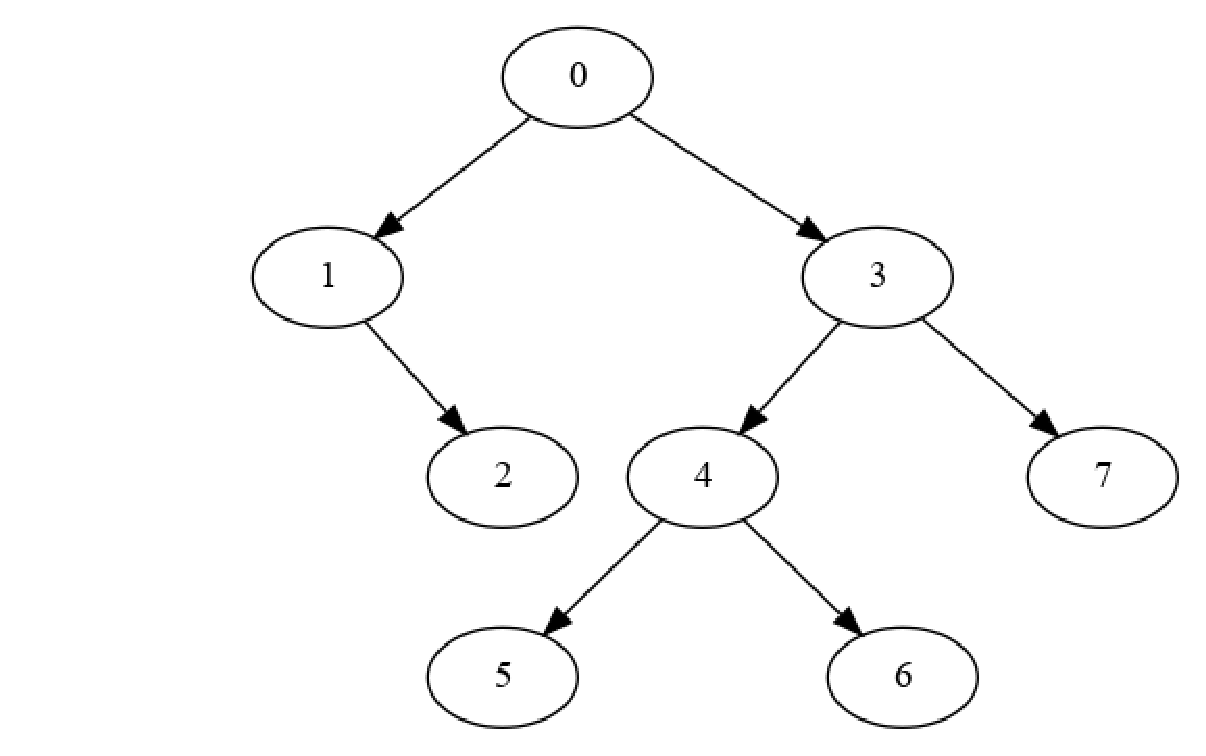
\includegraphics[width=200px]{sol.eps}
		\end{center}
	}
	\Question{Comment savoir si deux listes de valeurs correspondent aux parcours prefixe et infixe d'un arbre binaire ?}
	\tcor{On note $p = [p_0, \dots p_{n-1}]$ et $i = [i_0, \dots i_{n-1}]$ les listes représentant les parcours prefixe et infixe. Comme ce sont les parcours du même arbre, $i$ est une permutation de $p$. On extrait deux sous listes $i_g$ et $i_d$ de $i$, $i_g$ sont les éléments situés à gauche de $p_0$ et $i_d$ ceux situés à droite. On extrait de même deux sous listes de $p$, $p_g$ contient les $|i_g|$ éléments situés après $p_0$ et $p_d$ le reste de la liste. La liste $p_g$ doit être une permutation de $i_g$ et $p_d$ doit être une permutation de $i_d$. Et cette propriété doit rester vraie en reproduisant ce processus récursivement sur les deux listes extraites.}
	\Question{Ecrire une fonction qui prend en argument deux listes (le parcours prefixe et le parcours infixe) et qui renvoie l'arbre binaire correspondant. On supposera que les étiquettes de l'arbre sont des entiers tous différents.\\
		\aide \; On pourra commencer par écrire :
		\begin{itemize}
			\item Une fonction {\tt separe\_valeur} de signature {\tt int -> int list -> int list * int list} qui prend en argument un entier, une liste contenant cet entier et renvoie un couple de liste : les élément situés avant (resp après) cette valeur
			\item Une fonction {\tt separe\_nb} de signature {\tt int -> int list -> int list * int list} qui prend en argument un entier {\tt n} et une liste et renvoie un couple de listes : les {\tt n} éléments situés après le premier puis le reste de la liste.
		\end{itemize}
	}
	\tcor{\inputpartOCaml{reconstruction.ml}{}{}{75}{95}}

\end{Exercise}


\begin{Exercise}[title = {Expression bien parenthésée}]\\
	On considère dans cet exercice un parenthésage avec les couples $()$, $\{\}$ et  $[]$. On dira qu'une expression est bien parenthésée si chaque symbole ouvrant correspond à un symbole fermant et si l'expression contenue à l'intérieur est elle-même bien parenthésée.
	\Question{Les expressions suivantes sont-elles bien parenthésée ?
		\begin{itemize}
			\item[\textbullet] $3+[5-4\div(3+2)]\}+10$
			\item[\textbullet] $\{(3+2)\times 5$
			\item[\textbullet] $5)-4\times2($
			\item[\textbullet] $[(3+2)\times(5-3)]$
		\end{itemize}}
	\Question{Rappeler les fonctions de l'interface d'une pile.}
	\tcor{
		Structure de données séquentielle de type {\sc lifo} (dernier entré, premier sorti)
		\begin{itemize}
			\item Empiler (ajouter un élément au sommet de la pile)
			\item Dépiler (retirer l'élément situé au sommet de la pile)
			\item Est\_vide (qui permet de savoir si la pile est vide)
		\end{itemize}}
	\Question{Ecrire une fonction {\tt bien\_parenthesee} de signature {\tt str -> bool} qui renvoie {\tt true} lorsque la chaine de caractère donnée en argument est une expression bien parenthésée \\
		\aide \; on utilisera le module {\tt Stack} de OCaml afin de disposer d'une structure de pile \textit{mutable}. On rappelle ci-dessous les fonctions principales de ce module :
		\begin{itemize}
			\item \mintinline{ocaml}{Stack.create} de signature {\tt () -> 'a t} qui crée une pile vide d'éléments de type {\tt 'a}. Par exemple \mintinline{ocaml}{let mapile = Stack.create ()}
			\item \mintinline{ocaml}{Stack.push} de signature {\tt 'a 'a t -> ()} qui empile un élément. Par exemple \mintinline{ocaml}{Stack.push 5 mapile} empile l'entier 5 sur {\tt mapile} (le type option 'a est alors le type {\tt int}).
			\item \mintinline{ocaml}{Stack.pop} de signature {\tt 'a t -> 'a} qui renvoie l'élément situé au sommet de la pile en le dépilant.
		\end{itemize}
	}
	\tcor{\inputpartOCaml{bien_parenthesee.ml}{}{}{1}{29}}
\end{Exercise}

\begin{Exercise}
	\Question{Rappeler la définition du type abstrait \textit{file} et donner les fonctions de son interface.}
	\tcor{
		Structure de données séquentielle de type {\sc fifo} (premier entré, premier sorti)
		\begin{itemize}
			\item Enfiler (ajouter un élément à la file)
			\item Défiler (retirer un élément de la file)
			\item Est\_vide (qui permet de savoir si la file est vide)
		\end{itemize}}
	\Question{On rappelle que lorsque la file a une capacité bornée $N$, on peut l'implémenter en utilisant un tableau {\tt tab} de taille $N$ qu'on traite de façon circulaire. On maintient alors à jour :
		\begin{itemize}
			\item une variable {\tt size}  contenant le nombre d'élément de la file
			\item une variable {\tt next} contenant l'indice du prochain élément à défiler
		\end{itemize}
		Expliciter les opérations enfiler et défiler en terme de modification sur {\tt tab}, {\tt size} et {\tt next}.}
	\tcor{
		\begin{itemize}
			\item enfiler (on doit vérifier que la file n'est pas pleine en comparant {\tt size} et {\tt N}). En notant {\tt x} l'élément à enfiler et on affecte {\tt tab[(next+size)\%N]=x} et on incrémente {\tt size}.
			\item défiler on renvoie {\tt tab[next]}, on incrémente {\tt next} et on décrémente {\tt size}.
		\end{itemize}
	}

	\Question{Dans le cas où $N=3$, décrire le contenu de {\tt tab} et des variables {\tt size} et {\tt next} lorsqu'on effectue les opérations suivante : enfiler 2, enfiler 3, défiler, enfiler 4, défiler, enfiler 7, enfiler 8.}
	\tcor{
		\begin{tabular}{>{\tt}l|>{\tt}l|>{\tt}l}
			tab    & size & next \\
			\hline
			{[2] }   & 1    & 0    \\
			{[2; 3]} & 2    & 0    \\
			{[2; 3]} & 1    & 1    \\
            {[2; 3; 4]} & 2    & 1    \\
            {[2; 3; 4]} & 1    & 2    \\
            {[7; 3; 4]} & 2    & 2    \\
            {[7; 8; 4]} & 3    & 2    \\
		\end{tabular}
	}
	\Question{Donner une implémentation en OCaml en utilisant le type suivant :
		\inputpartOCaml{ringbuffer.ml}{}{}{1}{6}
	}
    \tcor{\inputpartOCaml{ringbuffer.ml}{}{}{8}{20}}
\end{Exercise}

\begin{Exercise}[title = {Comptine enfantine}]\\
	Certaines comptines enfantines ont pour objectif de désigner une personne \og{} au hasard \fg{}, un exemple bien connu est \og{} \textit{Am, stram, gram, pic et pic et colégram} \fg{}. On suppose que $N$ enfants numérotés de 0 à $N-1$ sont assis en cercle et que l'un d'entre eux (le numéro $k$) récite une comptine contenant $S$ syllabes. A la première syllable il désigne son suivant immédiat dans le cercle puis il avance d'un enfant à chaque syllable jusqu'à la fin de la comptine. L'enfant désigné à la fin de la comptine doit quitter le cercle et le processus recommence à partir de son suivant immédiat jusqu'à ce qu'un seul enfant reste.
	\Question{Donner une illustration de ce processus avec $N=5$ et $S=7$, en supposant que l'enfant $0$ commence.}
    \tcor{
        \begin{enumerate}
            \item[-] [0; 1; 2; 3; 4] 2 quitte le cercle et  3 récite la comptine
            \item[-] [0; 1; 3; 4] 1 quitte le cercle et  3 récite la comptine
            \item[-] [0; 3; 4] 4 quitte le cercle et  0 récite la comptine
            \item[-] [0; 4] 4 quitte le cercle
        \end{enumerate}
    }
	\Question{Implémenter en OCaml, un programme exécutant ce processus et donnant le numéro de l'enfant restant. On pourra utiliser 
    le module {\tt Queue} de OCaml. Dont on rappelle ci-dessous les fonctions principales :
		\begin{itemize}
			\item \mintinline{ocaml}{Queue.create}  qui crée une file vide d'éléments de type {\tt 'a}.
			\item \mintinline{ocaml}{Queue.add}  qui enfile un élément.
			\item \mintinline{ocaml}{Queue.take} qui défile
		\end{itemize}}
    \tcor{\inputpartOCaml{comptine.ml}{}{}{1}{16}}

\end{Exercise}

\begin{Exercise}[title = {Tester si un arbre est un {\sc abr}}]

	\Question{Rappeler la définition d'un arbre binaire de recherche}
    \tcor{Pour tous les noeuds de l'arbres, les valeurs du sous arbre gauche (resp. droit) sont strictement inférieures (resp. supérieures) à l'étiquette du noeud.}
	\Question{Proposer deux méthodes de complexité linéaire permettant de vérifier qu'un arbre est bien un {\sc abr}.}
    \tcor{
        \begin{itemize}
            \item Effectuer un parcours infixe de l'arbre en complexité linéaire et vérifier si la liste des valeurs obtenues est triée dans l'ordre croissant
            \item Parcourir l'arbre en donnant l'intervalle de valeurs dans lequel doit se trouver les éléments. Initialement l'intervalle est celui des entiers représentables, puis à chaque fois qu'on descend à gauche (resp. à droite) on met à jour la borne droite (resp gauche) de l'intervalle
        \end{itemize}
    }
	\Question{Donner l'implémentation de l'une au moins des méthodes.}
    \tcor{
		\begin{itemize}
			\item Méthode 1 : attention, le parcours infixe utilisant l'opérateur de concaténation de liste {\tt @} n'est \textit{pas} de complexité linéaire (la preuve a été faite en TD). On utilise ici un parcours infixe avec un accumulateur de façon à avoir une complexité linéaire. Il faut ensuite vérifier que la liste obtenue est triée.
			\inputpartOCaml{est_abr.ml}{}{}{94}{107}
			\item Méthode 2 : On initialise les deux bornes de l'intervalle dans lequel doivent se trouver les valeurs rencontrées avec le plus petit (\mintinline{ocaml}{Int.min_int}) et le plus grand (\mintinline{ocaml}{Int.max_int}) entier représentable.
			\inputpartOCaml{est_abr.ml}{}{}{109}{114}
		\end{itemize}
	}
\end{Exercise}


\begin{Exercise}[title = {Recherche dans un {\sc abr}}]
	\Question{Rappeler la définition d'un arbre binaire de recherche}
	\Question{On suppose maintenant qu'on a inséré dans un {\sc abr} initialement vide tous les entiers compris en 0 et 999. On effectue la recherche de l'entier 666 dans cet arbre. Parmi les séquences de valeurs suivantes, lesquelles peuvent être la séquence de noeuds parcourus jusqu'à  atteindre 666 ? :
		\begin{itemize}
			\item 487, 503, 911, 954, 499, 651, 672, 668, 666
			\item 951, 812, 803, 798, 751, 670, 589, 652, 653, 666
			\item 985, 112, 251, 306, 444, 503, 574, 602, 605, 681, 666
			\item 844, 511, 845, 603, 702, 651, 699, 660, 670, 665, 666
			\item 303, 404, 541, 752, 749, 742, 592, 603, 666
		\end{itemize}}
		\tcor{
		\begin{itemize}
			\item Non valide ! 487, 503, 911, 954, \textcolor{red}{499}, 651, 672, 668, 666 :
			\item Valide 951, 812, 803, 798, 751, 670, 589, 652, 653, 666
			\item Valide 985, 112, 251, 306, 444, 503, 574, 602, 605, 681, 666
			\item Non valide ! 844, 511, \textcolor{red}{845}, 603, 702, 651, 699, 660, 670, 665, 666
			\item Valide 303, 404, 541, 752, 749, 742, 592, 603, 666
		\end{itemize}}
	\Question{Proposer un algorithme qui prend en entrée une séquence d'entiers $u_0, \dots u_{n}$ avec $u_n$ la valeur cherchée et vérifie que cette séquence peut effectivement constituer la suite de noeuds visités lors de la recherche réussie d'un nombre dans un tel {\sc abr}. L'algorithme doit avoir une complexité temporelle en $O(n)$.}
	\tcor{Initialement, les valeurs rencontrées doivent être comprises en 0 et 999. Puis pour tout $i = 0 \dots n$, si $u_i$ est supérieure (resp. inférieure) à la valeur cherchée on met à jour la borne supéreure (resp. inférieure). On renvoie une erreur si la valeur n'est pas comprise entre les deux bornes}
	\Question{En fournir une implémentation en OCaml, en supposant que la séquence est donnée sous la forme d'un tableau d'entiers de OCaml. La signature de votre fonction sera donc {\tt int array -> bool}}
	\tcor{
		L'énoncé ne précise pas si la séquence est fournie sous forme de tableau ou de liste (laissé au choix de l'élève). Ci-dessous les corrections dans les deux cas de figure
		\inputpartOCaml{seq_search.ml}{}{}{1}{21}
	}
	\Question{Soit $t$ un tableau représentant la suite de valeurs obtenue lors de la recherche réussie d'un élément dans un {\sc abr}, proposer un algorithme \textit{de complexité linéaire} permettant de trier ce tableau. En donner l'implémentation en OCaml.}
	\tcor{De part la propriété des {\sc abr}, les valeurs inférieures à celle recherchée sont rangées dans l'ordre décroissante dans la séquence et les valeur supérieures à la valeur recherchée sont rangées dans l'ordre croissant. On parcourt donc la séquence en créant deux listes (les valeurs supérieures et inférieure à la valeur cherchée) et on concatene ensuite ces listes.
	\inputpartOCaml{seq_search.ml}{}{}{24}{29}
	On peut en donner une version un peu plus concise avec  :
	\inputpartOCaml{seq_search.ml}{}{}{31}{32}
	}
\end{Exercise}

\begin{Exercise}[title = {Collision dans une table de hachage}]\\
	Pour une chaine de caractères $s = c_0\dots c_{n-1}$, on considère la fonction de hachage :
	$$ h(s) = \sum_{i=0}^{n-1} 31^i \times c_i$$
	\Question{Calculer le hash de la chaine {\tt "AB"}.}
	\tcor{$31\times 65 + 66 = 2081$}
	\Question{Montrer qu'il existe deux chaines de caractères de longueur 2, formées de lettres minuscules (code 97 à 122) ou majuscules (code 65 à 90) et produisant la même valeur pour $h$.}
	\tcor{En notant $E = \intN{65}{90} \cup \intN{97}{122}$, on cherche $(a,b) \in E^2$ et $(a',b') \in E^2$ tels que : $(a,b) \neq (a',b')$ et $31a + b = 31a' + b'$. Cette équation se ramène à $b-b' = 31(a'-a)$. Donc $b-b'$ est un multiple non nul de 31. l'écart entre $b'$ et $b$ étant au maximum en valeur absolue de $122-65 =  57$ les seules possiblités sont :
	\begin{itemize}
		\item[\textbullet] $b-b' = 31$ et donc $a'-a=1$. Ce qui donne $a' = a + 1$ (donc $a'$ et $a$ sont dans le même intervalle) et $b' = b-31$ donc ils ne sont pas dans le même intervalle. On peut prendre par exemple la solution $a = 65$ donc $a'=66$ et $b = 97$ donc $b' = 66$ c'est-à-dire les chaines {\tt "Aa"} et {\tt "BB"}.
		\item[\textbullet] $b-b' = -31$ et donc $a'-a=-1$.  Ce qui donne $a' = a-1$ et $b' = b+31$, par exemple la solution $a=66$, $a'=65$, $b = 67$ et $b'=98$ convient (c'est-à-dire les chaines {\tt "BC"} et {\tt "Ab"})
	\end{itemize}}
	
	\Question{En déduire une façon de construire un nombre arbitraire de chaînes de caractères de longueurs quelconques ayant la même valeur pour la fonction $h$. \label{qu}}
	\tcor{En concaténant plusieurs chaines de caractères de longueur deux ayant le même hash on obtient des chaine de caractère de longueur paire arbitrairement grande et ayant le même hash. Par exemple (en utilisant les exemples de longueur deux donnés à la question précédente), {\tt "AaBC"} et {\tt "BBAb"}. Pour la longueur impaire on rajoute le même caractère aux deux chaines.}
	\Question{Pour implémenter cette fonction en langage C, on propose une fonction de signature \mintinline{c}{int hash(char *s)}. Qu'en pensez-vous ?}
	\tcor{Les chaines de caractères "connaissent" leur longueur en C grâce au caractère sentinelle, on a donc pas besoin de passer la longueur de la chaine de caractère en paramètre. Par contre, cette fonction risque fort de provoquer un dépassement de capacité sur le type {\tt int} ce qui est un comportement indéfini en C. On devrait plutôt utiliser la librairie {\tt stdint.h} et renvoyer un {\tt uint}}
	\Question{Proposer une implémentation \textit{efficace} pour cette fonction en langage C.}
	\tcor{
	Le calcul par la méthode de Horner est de complexité linéaire (car évite le calcul explicite des puissances de 31)	
	\inputpartC{hash.c}{}{}{4}{14}}
	\Question{Déterminer, grâce à la question \ref{qu}, deux chaines de 8 caractères produisant une collision et le vérifier.}
	\tcor{
	On peut simplement deux chaines de longueur 4 ayant le même hash avec elle-même :
	\inputpartC{hash.c}{}{}{16}{22}
	}
\end{Exercise}


\end{document}